\documentclass[a4paper]{article}

%% Language and font encodings
\usepackage[english]{babel}
\usepackage[utf8x]{inputenc}
\usepackage[T1]{fontenc}

%% Sets page size and margins
\usepackage[a4paper,top=3cm,bottom=2cm,left=3cm,right=3cm,marginparwidth=1.75cm]{geometry}

%% Useful packages
\usepackage{amsmath}
\usepackage{graphicx}
\usepackage[colorinlistoftodos]{todonotes}
\usepackage[colorlinks=true, allcolors=blue]{hyperref}

\usepackage[authoryear]{natbib}

%% My definition
\newcommand{\toshi}{\textcolor{blue}}
\newcommand{\laurie}{\textcolor{red}}
\newcommand{\rishi}{\textcolor{green}}
\newcommand{\iago}{\textcolor{purple}}

\newcommand{\disp}{\displaystyle}

\usepackage{enumitem}
https://www.overleaf.com/project/5ca9fed01e2a625dbaeae31f
\usepackage{algorithm}
\usepackage{algorithmicx}
\usepackage{algpseudocode}

\usepackage{color}
\definecolor{darkgreen}{rgb}{0.0, 0.5, 0.0}
\definecolor{darkred}{rgb}{0.7, 0.11, 0.11}
\definecolor{darkblue}{rgb}{0,0,0.5}
\definecolor{shadecolor}{rgb}{1,1,0.95}
\definecolor{shade}{rgb}{1,1,0.95}
\definecolor{coilin}{rgb}{1,0,1}

\newcommand{\laurie}{\textcolor{darkred}}
\newcommand{\toshi}{\textcolor{darkblue}}
\newcommand{\rishi}{\textcolor{darkgreen}}
\newcommand{\todo}[1]{\laurie{\textbf{\textit{#1}}}}


\title{Is It You or Your Model Talking}
\author{Laurie Kell, Toshihide Kitakado, Rishi Sharma, ...}

\begin{document}
\maketitle

\newpage       
\section*{Outline}

\begin{itemize}
    \item To provide fisheries management advice requires predicting the response of a stock to management and checking that the predictions are consistent with reality (pers. com. Sidney Holt). The accuracy and precision of predictions depend on the validity of the model, the information in the data, and how far ahead we wish to predict. 
    \item Often in stocks assessment multiple models with different structures and datasets, are used to explore uncertainty. This means that it is difficult to compare models using conventional metrics such as AIC.  
    \item We therefore used prediction skill to validate models across families i.e. SS, SS-ASPM, and Jabba for Indian Ocean yellowfin tuna. 
    \item Retrospective analyses are commonly used to evaluate the stability of stock assessment estimates, however, stability can be at the expense of prediction skill, i.e. by using shrinkage.
    \item We therefore predict forward from retrospective analysies and then compare model predictions with historical estimates.
    \item It is not possible, however, to validate models based on model outputs we therefore conduct model free hindcasts, and MASE to compare observations with model estimates. This allows us to compare different data components and model to explore data conflicts and potential model misspecification.
    \item We also address the question what do you when you have a model with high MASE score and/or mohn’s rho? i.e. a retropective analysis while useful is not sufficient as we can only validate models based on observations.
    \item  We discuss the use of multiple metrics and the consequences for MSE, i.e. for weighting OMs and developing OEMs    
    \item How to expand the hindcast to include a jackknife to estimate prediction residuals, and perform the hindcast by series.
\end{itemize}

\tableofcontents 

\newpage
\begin{abstract}
    Evaluating how well the model fits data has been receiving much attention in fisheries science, both in terms of goodness-of-fit and retrospectively. This however merely tells us how well we can describe the past, yet little how well we can predict the future under alternative management actions. In this paper, we revisit the concepts behind hindcasting cross-validation (hcxval) as an important model-free validation tool for predictive modelling. Together with conventional residual diagnostics and retrospective analysis, we apply hcxval to three examples of alternative candidate models using the recent Indian Ocean yellowfin tuna assessment as a case study. 
    These models comprise the 2019 spatially structured reference model implemented in Stock Synthesis (ss-ref), a deterministic age-structured production model (ss-aspm) of ss-ref and a simplied spatially aggregated stochastic surplus production model implemented in the 'JABBA' package. To assess prediction skill, we computed the Mean-Absolute-Scaled-Error (MASE), which, unlike e.g. Aikaike's Information Criterion, enables to compare across different models fitted different data. The best MASE values (MASE < 1) were determined for ss-asem, which indicates that recruitment deviations in ss-ref were poorly estimated due to no or limited information in the 'noisy' length composition data. By contrast, the area effects retained in ss-aspm best explained its superior prediction skill compared to the spatially aggregated jabba model. We suggest that one-step ahead predictions are efficient for detecting overfitting and for model validation in general, but for future quota advice the forecast horizon should preferably at least match the assessment interval to ultimately increase confidence in the model-based scientific advice by stake holder and managers and policy makers.
\end{abstract}
   
\section{Introduction}

In stock assessment most goodness of fit diagnostic are based on residuals obtained from fits to historical observations. To provide fisheries management advice, however, requires predicting the response of a stock to management and checking that the predictions are consistent with reality (pers. com. Sidney Holt). The accuracy and precision of predictions depend on the validity of the model, the information in the data, and how far ahead we wish to predict. Validation examines if a model should be modified or extended and is complementary to model selection and hypothesis testing. Model selection searches for the most suitable model within a family, whilst hypothesis testing examines if the model structure can be reduced.

Model validation is important in many fields, e.g. in energy and climate models, as it increases confidence in the outputs of a model and leads to an increase in trust amongst the public, stake and asset-holders and policy makers \citep{kellSubmitted}. For models to be valid they must satisfy four prerequisites \citep{hodge1992}, the situation being modelled must be observable and measurable, it must be possible to collect sufficient data, exhibit constancy of structure in time, and exhibit constancy across variations in conditions not specified in the model. The first two prerequisites should be straight forward but for highly migratory stocks fished in areas beyond national jurisdiction (ABNJ) most stock assessments depend on fisheries dependent data rather than scientific observation. Prerequisite 3 ensures that the model has predictive skill for the same conditions under which the validation tests were conducted, and 4 that the model will still be valid for conditions that differ from those in the validation tests. In the later case this means can the model be used to set robust management advice. 

To explore the robustness of advice to uncertainty requires different model structures to be condition on alternative and potentially conflicting datasets. In such cases model selection criteria such as AIC, however, cannot be applied. The first prerequisite of means it is not possible to validate a model, using derived quantities, such as SSB and F. An alternative is to use model-free hindcasting, a form of crossvalidation where observations are compared to their predicted values. The key concept in this case is prediction skill, defined as any measure of accuracy of a forecasted value to the actual (i.e. observed) value that is not known by the model \cite{Huschke1959}.

To illustrate the utility of hindcasting we develop a case study based on bigeye and yellowfin tuna stocks in the Indian, Atlantic and Eastern Pacific Oceans, and four assessment methods, SS, SS-ASPM, Jabba-Select and Jabba. 

\section{Material and Methods}

\cite{kell2016xval} proposed a model-free hindcasting using crossvalidation where observations (e.g. CPUE) are compared to their predicted future values. The hindcasting algorithm is similar to that used in retrospective analysis \citep{Hurtado2014, carvalho}, which involves sequentially removing  observations from the terminal year (peels), fitting the model to the truncated series, and then comparing the difference between model estimates from the truncated time-series to those estimated using the full time series. In a model-free hindcast an additional step is included, i.e. projecting over the missing years and then cross-validating these forecasts against observations to assess the model’s prediction skill.

\subsection{Assessment Methods}

Case study based on Indian Ocean yellowfin tuna stocks and four assessment methods, SS, SS-ASPM, Jabba-Select and Jabba. 

\begin{verbatim}%
There has been a recent trend in stock assessment to use integrated analysis that combines several sources of data into a single model by a joint likelihood for the observed data (Doubleday, 1976, Fournier and Archibald, 1982, Maunder and Punt, 2013).  Datasets include records of catches and landings, indices of abundance based on catch per unit (CPUE) and from research surveys, and the length classes and/or ages compositions based on samples. A commonly used integrated assessment method is Stock Synthesis (Methot and Wetzel, 2013) that can be configured in multiple ways e.g. SSS and ASPM.

Alternatives are biomass dynamic models based on a surplus production function that requires the estimation or fixing of fewer parameters, since many parameters required in integrated assessments are difficult to estimate in practice (e.g. Lee et al.). Once such example is JABBA an open source package that presents a unifying, flexible framework for biomass dynamic modelling, runs quickly, and generates https://www.overleaf.com/project/5ca9fed01e2a625dbaeae31freproducible stock status estimates.

A problem is how to compare these different models


\begin{description}
\item{SS} 
Stock Synthesis (Methot and Wetzel 2013; SS) is widely used to perform integrated assessments for fish stocks in the United States and throughout the world. While Stock Synthesis is typically applied in data-rich circumstances, its use in data-moderate stock assessments (where catch time series and abundance indices are available, and catch composition data is limited or absent) has significantly increased in recent years. The uptake of Stock Synthesis for integrated data-moderate stock assessments has occurred especially in assessments developed for Regional Fishery Management Organizations (RFMOs). Various stocks of billfish and pelagic sharks that were historically assessed using Surplus Production Models and Virtual Population Analysis (VPA) are now moving towards full implementation in Stock Synthesis as additional data become available (e.g. Courtney et al. 2017; Schirripa 2019). Similarly, there has been a recent increase in Stock Synthesis benchmark assessment in Europe in place of the conventionally used VPA with extended survivor analysis (XSA) in the region (Max Refs). The visualization of model outputs and implementation of diagnostics for Stock Synthesis is facilitated by the availability of a comprehensive collection of R functions (r4ss; https://github.com/r4ss).

\item{ASPM} 
Maunder and Piner (2015) proposed the ASPM age-structured production model (ASPM) as a diagnostic of process dynamics. This diagnostic evaluates whether the observed catches alone (taken out of approximately the correct ages) can explain trends in the index of abundance. On the one hand, Maunder and Piner (2015) suggest that if the ASPM is able to fit well to the indices of abundance that have good contrast (i.e. those that have declining as well as increasing trends), the production function likely exists, and the indices will provide information about absolute abundance. On the other hand, the authors suggest that if there is not a good fit to the indices, then the catch data alone cannot explain the trajectories depicted in the indices of relative abundance. This can have several causes: (i) the stock is recruitment-driven; (ii) the stock has not yet declined to the point at which catch is a major factor influencing abundance; (iii) the base-case model is incorrect; or (iv) the indices of relative abundance are not proportional to abundance. Alternatively, failure in the ASPM may indicate a system that is not well organized (e.g., stock structures or data are incorrect) so that a real fishing signal is lost or where unknown environmental drivers control population abundance. The ASPM was shown via simulation analyses to be the only tested diagnostic capable of detecting misspecification of the key systems-modeled processes that control the shape of the production function (Carvalho et al., 2017).
\item{Jabba}
This study presents a new, open-source modelling software entitled ‘Just Another Bayesian Biomass Assessment’ (JABBA). JABBA can be used for biomass dynamic stock assessment applications, and has emerged from the development of a Bayesian State-Space Surplus Production Model framework, already applied in stock assessments of sharks, tuna, and billfishes around the world. JABBA presents a unifying, flexible framework for biomass dynamic modelling, runs quickly, and generates reproducible stock status estimates and diagnostic tools. Specific emphasis has been placed on flexibility for specifying alternative scenarios, achieving high stability and improved convergence rates. Default JABBA features include: 1) an integrated state-space tool for averaging and automatically fitting multiple catch per unit effort (CPUE) time series; 2) data-weighting through estimation of additional observation variance for individual or grouped CPUE; 3) selection of Fox, Schaefer, or Pella-Tomlinson production functions; 4) options to fix or estimate process and observation variance components; 5) model diagnostic tools; 6) future projections for alternative catch regimes; and 7) a suite of inbuilt graphics illustrating model fit diagnostics and stock status results. As a case study, JABBA is applied to the 2017 assessment input data for South Atlantic swordfish (Xiphias gladius). We envision that JABBA will become a widely used, open-source stock assessment tool, readily improved and modified by the global scientific community.
\end{description}\end{verbatim}

\subsection{Procedure}

\subsubsection{Retrospective}

\begin{verbatim}%include{retro.tex}\end{verbatim}

\subsubsection{Hindcast} 

\begin{verbatim}%include{hindcast.tex}\end{verbatim}

\subsection{Summary Metrics}

\begin{verbatim}%include{metrics.tex}\end{verbatim}

\section{Results}

Figure~\ref{fig:map} shows the stock distribution shows the stock structure assumed in the SS assessments.

The first step was to conduct a retrospective analysis and the estimates of stick biomass (SSB for ASPM and SS, and biomass for JABBA) and F (instantaneous for ASPM and SS, and rate for JABBA) are shown in Figure~\ref{fig:retro}. The terminal estimates were then project forward for three years assuming the reported catches and the estimated recruitment from the model with all years included  (Figure~\ref{fig:predictions}). ASPM "predicted" values are close to those of the assessment that includes all years. For SS, however, there is a large overestimation of future biomass, and a underestimate of F . For JABBA the strongest retrospective pattern is seen in F, which is underestimated in the predictions.

The residuals from the model fits are shown in Figure~\ref{fig:runs}, the backgroud indicates whether they passed (green) or failed (red) the runs tests. 

The results from the model-free  Hindcast with one year ahead predictions are shown in Figure~\ref{fig:hy1} and from the three year ahead predictions in Figure~\ref{fig:hy3}.

Figure~\ref{fig:runshat} shoes the predictions residuals, and the fits are summarised in Figures~\ref{fig:td} and Figure~\ref{fig:tdhat} in the form of Taylor diagrams

\subsection*{Summary}

\begin{description}
    \item{Retrospective analysis and projections for F/FMSY and B/BMSY} show that
    \begin{itemize}
        \item SS projections and hence advice is based upon SS is unreliable.
        \item Jabba advice is problematic as it appears that even if F<FMSY the stock will decline below BMSY
        \item ASPM appears consistent
        \item It therefore appears that the length compositions just add noise, and that area effects are important
        \item However these is no objective way to choose an assessment based on retrospective analysis as the best model would always be B/MSY = 1 
        \end{itemize}
    \tem{Model-free cross-validation} confirms the relative performance of the models
    \begin{itemize}
        \item ASPM performs best
        \item Survey 2 performs poorly across all models
   \end{itemize}
   \item{Make case for why we need MASE and why this new methodology is important}
    \begin{itemize}
        \item Tabulate Metrics
        \item Compare MASE to other measures and use Taylor Diagrams to explain differences
   \end{itemize}

\end{description}

\section{Discussion}

\begin{verbatim}%include{discussion.tex}\end{verbatim}
\section{Conclusions}


Primary objectives were:
\begin{enumerate}
    \item Unifying platform for evaluating across models
    \item Advantage of MASE : What are the new properties of this stat
    \item In fisheries unlike other fields we try to account for the past but not for the future. Here we propose a way to assess model predictive performance and to account for alternative models within a common diagnostic framework.
\end{enumerate}


\bibliographystyle{apalike}
\bibliography{/home/laurence/Desktop/sea++/xval/manuscripts/peerReview/refs.bib}

\section{Tables}

\section{Figures}

\begin{figure*}[htbp]
\centering
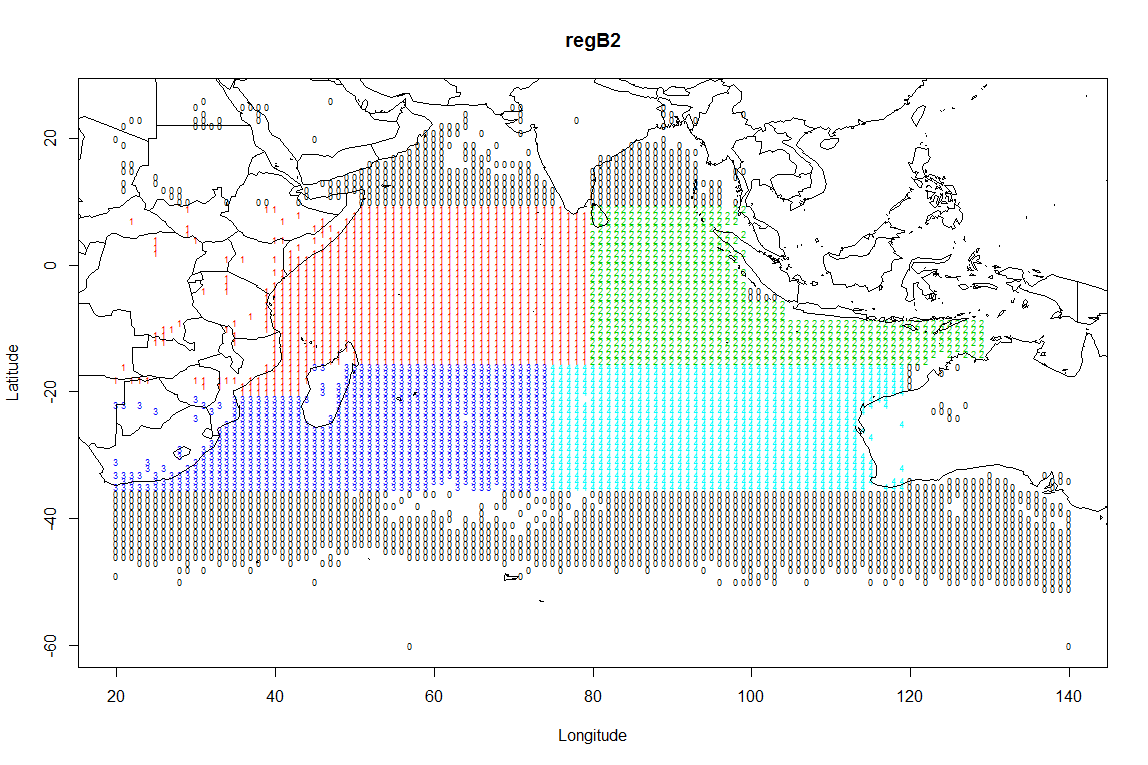
\includegraphics[width=6in]{map.png}
\caption{Stock distribution.}
\label{fig:map}
\end{figure*}

\begin{figure*}[htbp]
\centering
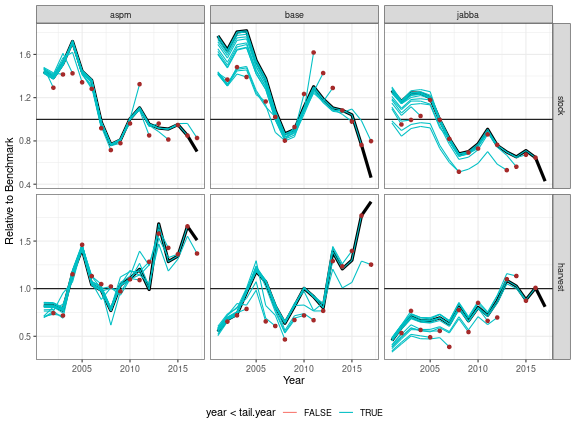
\includegraphics[width=6in]{final-retro-1.png}
\caption{Retrospective analysis for the three models, points indicate the terminal years, and the think line the assessment using all the data.}
\label{fig:retro}
\end{figure*}

\begin{figure*}[htbp]
\centering
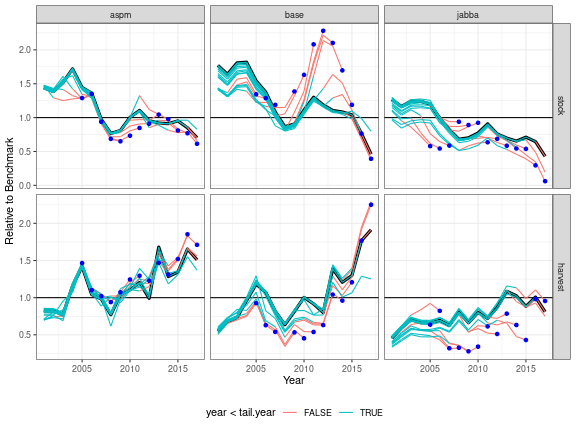
\includegraphics[width=6in]{final-retro3-1.png}
\caption{Retrospective analysis with three year predictions for the three models, points indicate the terminal years, and the think line the assessment using all the data.}
\label{fig:predictions}
\end{figure*}


\begin{figure*}[htbp]
\centering
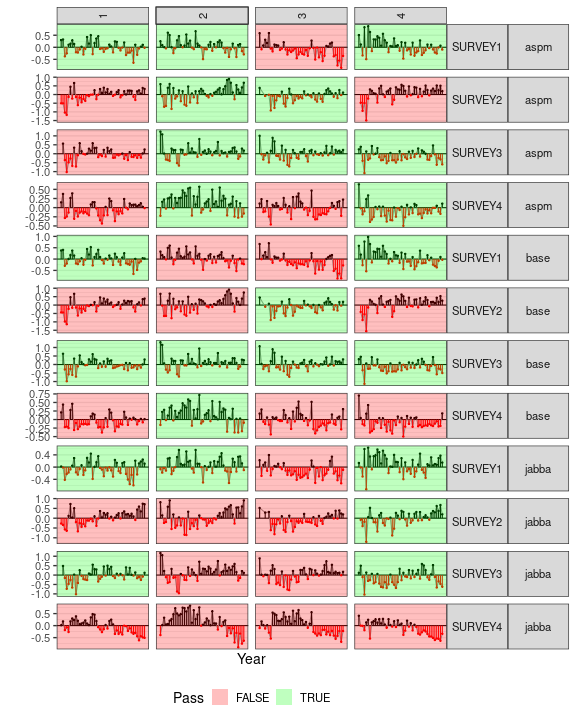
\includegraphics[width=6in]{final-cpue-residual-runs-1.png}
\caption{Residual runs tests for fits to the three models; green background indicates series where runs tests are passed.}
\label{fig:runs}
\end{figure*}

\begin{figure*}[htbp]
\centering
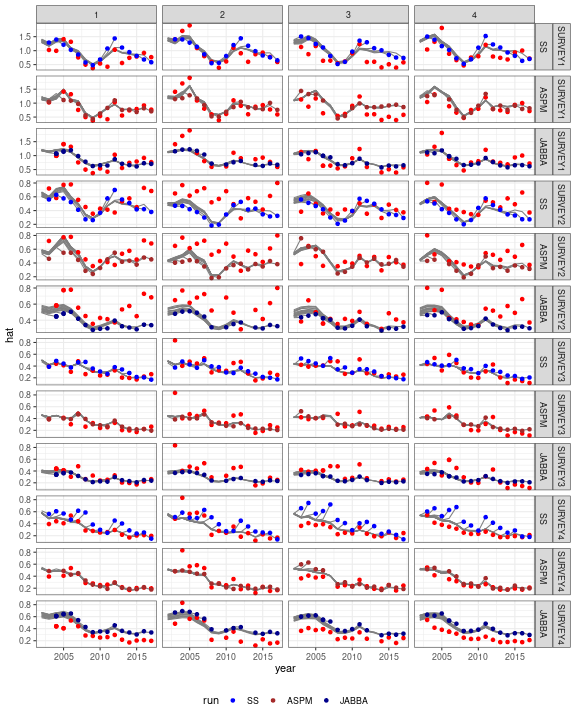
\includegraphics[width=6in]{final-hy-plot-1.png}
\caption{Hindcast with one year ahead predictions, red dots are the observed CPUE values and lines are the fits with terminal hincast year indicated by a point.}
\label{fig:hy1}
\end{figure*}

\begin{figure*}[htbp]
\centering
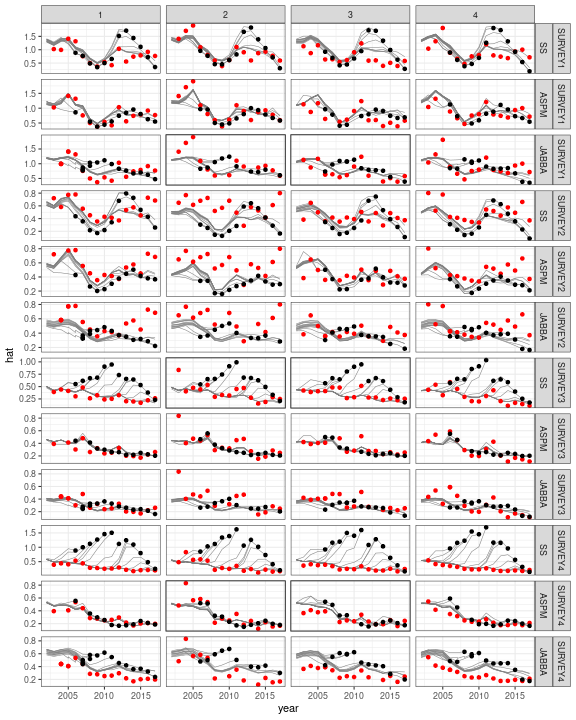
\includegraphics[width=6in]{final-hy3-plot-1.png}
\caption{Hindcast with three year ahead predictions, red dots are the observed CPUE values and lines are the fits with terminal hincast year indicated by a point.}
\label{fig:hy3}
\end{figure*}


\begin{figure*}[htbp]
\centering
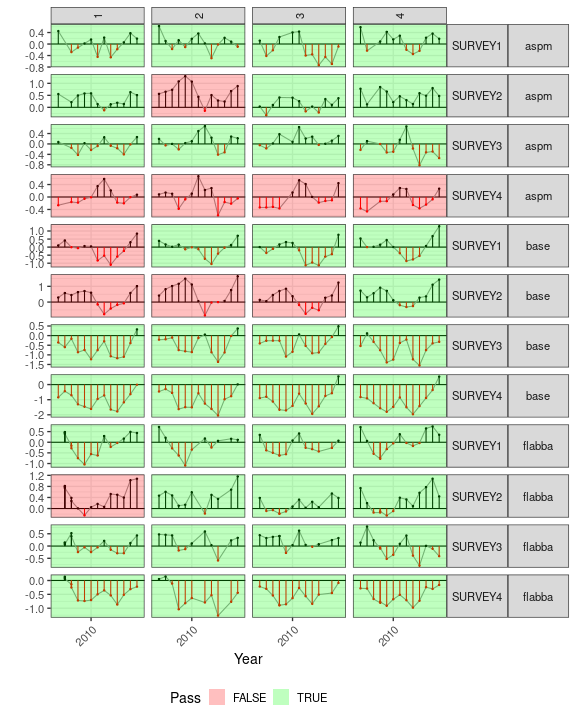
\includegraphics[width=6in]{final-cpue-prediction-runs-1.png}
\caption{Runs tests for one step ahead residuals.}
\label{fig:runshat}
\end{figure*}


\begin{figure*}[htbp]
\centering
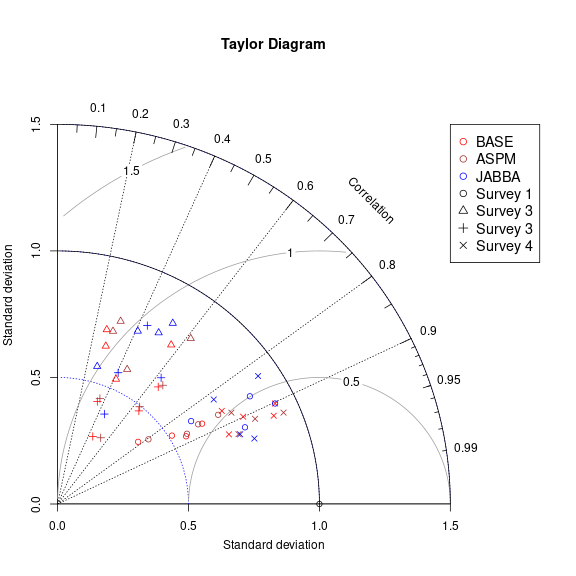
\includegraphics[width=6in]{final-taylor-residuals-1.png}
\caption{Taylor diagram for fits to CPUE summarising the similarity between the observed time series of CPUEs and the predicted relative stock abundance. Each point quantifies how closely predictions match observations, the angle indicates the correlation, the centred root-mean-square error difference between the predicted and observed patterns is proportional to the distance to the point on the x and the contours around this point indicate the RMSE values; the standard deviations of the predictions are proportional to the radial distance from the origin, scaled so the observed pattern has a value of 1. The open circle corresponds to a series which is identical to the reference series. The colours correspond to the model and shape to the survey.)}
\label{fig:td}
\end{figure*}

\begin{figure*}[htbp]
\centering
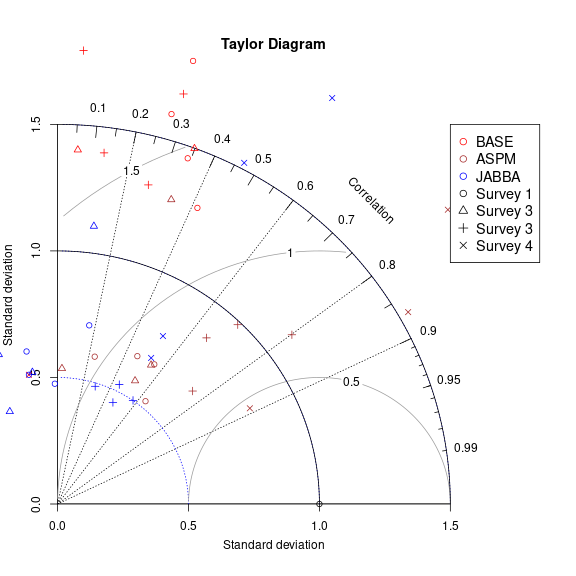
\includegraphics[width=6in]{final-taylor-hy-1.png}
\caption{Taylor diagram for 3 year ahead predictions, summarising the similarity between the observed time series of CPUEs and the predicted relative stock abundance. Each point quantifies how closely predictions match observations, the angle indicates the correlation, the centred root-mean-square error difference between the predicted and observed patterns is proportional to the distance to the point on the x and the contours around this point indicate the RMSE values; the standard deviations of the predictions are proportional to the radial distance from the origin, scaled so the observed pattern has a value of 1. The open circle corresponds to a series which is identical to the reference series. The colours correspond to the model and shape to the survey.}
\label{fig:tdhat}
\end{figure*}


%\begin{figure*}[htbp]
%\centering
%\includegraphics[width=6in]{final-cpue-plot-1.png}
%\label{fig:cpue}
%\caption{}
%\end{figure*}


\end{document}


\end{document}